\documentclass[a4paper, openany, 12pt]{article}

%% подключаем стандарт библиографии
\bibliographystyle{gost71u}

%% для "Abstract" в классе book
% \newenvironment{abstract}{}{}
% \usepackage{abstract}

%% подключаем преамбулу: в ней содержится подключение всех необходимых пакетов
%% Работа с русским языком
\usepackage{cmap}			 % поиск в PDF
\usepackage{mathtext} 		 % русские буквы в формулах
\usepackage[T2A]{fontenc}	 % кодировка
\usepackage[utf8]{inputenc}	 % кодировка исходного текста
\usepackage[russian]{babel}	 % локализация и переносы
\usepackage[percent]{overpic}
\usepackage{color}
\usepackage{subcaption}
\usepackage{svg}
\usepackage{listings}
\usepackage{xcolor}
\usepackage{setspace}

\lstdefinestyle{cppstyle}{
    language=C++,
    backgroundcolor=\color{gray!10},
    commentstyle=\color{green!60!black},
    keywordstyle=\color{blue}\bfseries,
    numberstyle=\tiny\color{gray},
    stringstyle=\color{red},
    basicstyle=\ttfamily\footnotesize,
    breakatwhitespace=false,
    breaklines=true,
    captionpos=b,
    keepspaces=true,
    numbers=left,
    numbersep=5pt,
    showspaces=false,
    showstringspaces=false,
    showtabs=false,
    tabsize=2,
    frame=single,
    framesep=3pt,
    xleftmargin=17pt,
    framexleftmargin=17pt,
    framexrightmargin=5pt,
    framexbottommargin=4pt,
    showlines=true
}

\lstset{style=cppstyle}


%% Пакеты для работы с математикой
\usepackage{amsmath,amsfonts,amssymb,amsthm,mathtools}
\usepackage{icomma}

%% Нумерация формул (опционально)
%\mathtoolsset{showonlyrefs=true} % показывать номера только у тех формул, на которые есть \eqref{} в тексте.
%\usepackage{leqno}               % нумерация формул слева

%% Шрифты
\usepackage{euscript}	 % шрифт "Евклид"
\usepackage{mathrsfs}    % красивый мат. шрифт

%% Некоторые полезные макросы для дебага (в случае недоверия авторам шаблона)
\makeatletter
\newcommand\thefontsize{The current font size is: \f@size pt} % пример: \section{\thefontsize}
\makeatother

%% Настройка размеров шрифтов
\makeatletter
\setlength{\headheight}{28pt}
%% TODO: мне не удалось разобраться, как грамотно подбирать второе число в
%% \@setfontsize\*, но ряд эксппериментов показывает, что "10" выравнивает текст весьма прилично :)
\renewcommand\Huge{\@setfontsize\Huge{14pt}{10}}
\renewcommand\huge{\@setfontsize\huge{14pt}{10}}
\renewcommand\Large{\@setfontsize\Large{14pt}{10}}
\renewcommand\large{\@setfontsize\large{12pt}{10}}
\makeatother

%% Поля (геометрия страницы)
\usepackage[left=3cm,right=1.5cm,top=2cm,bottom=2cm,bindingoffset=0cm]{geometry}

%% Русские списки
\usepackage{enumitem}
\makeatletter
\AddEnumerateCounter{\asbuk}{\russian@alph}{щ}
\makeatother

%% Работа с картинками
\usepackage{caption}
\captionsetup{justification=centering} % центрирование подписей к картинкам
\usepackage{graphicx}                  % вставки рисунков
\graphicspath{{images/}{images2/}}     % папки с картинками
\setlength\fboxsep{3pt}                % отступ рамки \fbox{} от рисунка
\setlength\fboxrule{1pt}               % толщина линий рамки \fbox{}
\usepackage{wrapfig}                   % обтекание рисунков и таблиц текстом

%% Работа с таблицами
\usepackage{array,tabularx,tabulary,booktabs} % дополнительная работа с таблицами
\usepackage{longtable}                        % длинные таблицы
\usepackage{multirow}                         % слияние строк в таблице

%% Красная строка
\setlength{\parindent}{2em}

%% Интервалы
\linespread{1}
\usepackage{multirow}

%% TikZ
\usepackage{tikz}
\usetikzlibrary{graphs,graphs.standard}

%% Верхний колонтитул
\usepackage{fancyhdr}
\pagestyle{fancy}

%% Перенос знаков в формулах (по Львовскому)
\newcommand*{\hm}[1]{#1\nobreak\discretionary{}{\hbox{$\mathsurround=0pt #1$}}{}}

%% Дополнительно
\usepackage{float}   % добавляет возможность работы с командой [H] которая улучшает расположение на странице
\usepackage{gensymb} % красивые градусы
\usepackage{caption} % пакет для подписей к рисункам, в частности, для работы caption*
\usepackage{listings} % пакет для листингов с кодом
\lstset{              % настройки для лисингов с кодом
basicstyle=\small\ttfamily,
columns=flexible,
breaklines=true
}

% Hyperref (для ссылок внутри  pdf)
\usepackage[unicode, pdftex]{hyperref}

% Отступ перед первым абзацем в каждом разделе
\usepackage{indentfirst}


\begin{document}
    %% титульник
    \begin{center}
    %% *название института*
    \large\textbf{Министерство образования и науки Российской Федерации \\
    Московский физико-технический институт (государственный
    университет)} \\
    \vspace{1cm}

    %% *факультет/физтех-школа*
    Физтех-школа радиотехники и компьютерных технологий \\

    %% *название базовой кафедры и лаборатории*
    %% в случае ненадобности можно удалить
    Кафедра микропроцессорных технологий в интеллектуальных системах управления \\

    \vspace{3em}

    Выпускная квалификационная работа бакалавра
\end{center}

\begin{center}
    \vspace{\fill}
    %% *название вашей работы*
    \LARGE{Профилирование и аннотация времени выполнения в MLIR как инструмент для оптимизации программ машинного обучения}

    \vspace{\fill}
\end{center}


\begin{flushright}
    \textbf{Автор:} \\
    Студент 109 группы \\
    Алексеев Алексей Алексеевич \\
    \vspace{2em}
    \textbf{Научный руководитель:} \\
    Черноног Вячеслав Викторович \\
    \vspace{2em}
    \textbf{Научный консультант:} \\
    Голенев Александр Дмитриевич \\
\end{flushright}

\vspace{7em}

\begin{center}
    %% *лого*
    
\includegraphics[width=100 pt]{MIPT_logo.jpg}\\
    Москва \the\year{}
\end{center}

%% выключаем отображение номера для этой страницы (титульник)
\thispagestyle{empty}

\newpage
\setcounter{page}{2}
\fancyfoot[c]{\thepage}
%% *надпись над верхним колонтинулом*
%% в случае ненадобности можно удалить
\fancyhead[R]{}
    %% аннотоция
    \begin{abstract}

    \begin{center}
        \large{Профилирование и аннотация времени выполнения в MLIR как инструмент для оптимизации программ машинного обучения} \\
    \large\textit{Алексеев Алексей Алексеевич} \\[1 cm]

    Современные модели машинного обучения представляют собой важнейшую область как для фундаментальных исследований, так и для решения прикладных задач в различных областях.
    Одной из актуальных задач в индустрии является создание инфраструктуры, которая позволит эффективно запускать и исполнять эти модели на устройствах с ограниченными ресурсами, на неоднородных и специализированных архитектурах.

    Моя работа направлена на решение проблемы формализации подхода к поиску возможных мест для оптимизаций моделей во время компиляции.
    Этот подход учитывает специфику выполнения программ на различных устройствах.
    Для достижения этой цели используются инструменты многоуровневого промежуточного представления (MLIR), а также динамические профили исполнения программ.

    В рамках работы была разработана система автоматического аннотирования промежуточного представления.
    Эти аннотации могут служить основой для применения дальнейших трансформаций и анализа, что позволит значительно ускорить выполнение программ машинного обучения.

    \vfill
    \end{center}


\end{abstract}
\newpage
    %% содержание
    \tableofcontents{}
    \newpage

    \fontsize{14}{16}\selectfont
    \setstretch{1.5}
    \section{Введение}
\label{sec:Chapter0} \index{Chapter0}

\subsection{Особенности задач машинного обучения}

За последние несколько лет методы машинного обучения (ML, от Machine Learning) продемонстрировали стремительный рост как в области применения, так и в качестве получаемых результатов.
В большинстве случаев этот прогресс стал возможен благодаря увеличению вычислительных мощностей используемых исполняющих сред.
Чтобы в полной мере оценить масштаб произошедших изменений, необходимо рассмотреть вычислительные требования, предъявляемые современными моделями, а также проанализировать особенности архитектур, на которых они исполняются.
Каждая модель машинного обучения условно делится на два этапа: обучение и использование (инференс).
Этап обучения заключается в подаче большего количества разнообразных примеров, на основе которых модель адаптирует свои параметры, чтобы повысить способность к обобщению и точности предсказаний на новых, ранее не виденных данных.
Этот процесс достигается с помощью математических методов регрессии и оптимизации, таких как поиск локального минимума в многомерном параметрическом пространстве.
Целью является построение модели, приближённой к оптимальной для заданного распределения входных данных.
Характерной чертой большинства таких задач является возможность их формализации с использованием примитивов линейной алгебры.
В упрощённом виде модель можно представить как последовательность алгебраических операций над тензором параметров $X$ и входными данными $F$, где $F$ представляет собой пространство признаков, а $Y$ — соответствующее пространство ответов.
Результатом обучения является набор параметров (весов) $X$, таких, что выполняется следующее условие:

\begin{equation}
|XF - Y|_{\text{norm}} \rightarrow \min
\end{equation}

На этапе инференса модель применяется к новым данным. Это означает сохранение последовательности алгебраических операций (часто представляемых в виде графа) и загрузку ранее полученных значений параметров $X$ на конечное устройство.
В отличие от обучения, инференс не включает в себя процесс оптимизации — он лишь выполняет предсказание на основе уже обученных весов, что делает его значительно менее ресурсоёмким.
Тем не менее, в последние годы наблюдается постоянное увеличение размера моделей, выражающееся как в количестве параметров, так и в сложности вычислений. Это ставит под вопрос возможность стабильной и быстрой работы моделей на конечных устройствах без потери качества или увеличения времени отклика.
На рисунке ниже представлена экспоненциальная тенденция роста количества операций при обучении современных моделей.
Этот рост напрямую коррелирует с вычислительной нагрузкой при их инференсе. Наблюдаемая зависимость в некотором смысле напоминает закон Мура, с той разницей, что вместо количества транзисторов речь идёт о росте размеров тензоров и значений их элементов.
Но за счёт чего физически компенсируется постоянно растущая сложность современных ML-моделей?

\begin{figure}[h]
\centering
\begin{overpic}[width=0.8\textwidth]{models_complexity.png}
\end{overpic}
\caption{Рост вычислительных требований при обучении современных моделей.}
\end{figure}

Вычислительно, процесс получения предсказания модели можно представить как последовательность вложенных циклов for, где каждая последующая строка соответствует проекции i-й координатной оси на итерационное пространство.
Подобная схема требует максимальной загрузки вычислительных ресурсов (CPU, GPU, NPU — подробнее о них ниже), что влечёт за собой значительные накладные расходы, включая потребление электроэнергии.
Вычислительные устройства можно условно расположить по шкале "приспособленности" к выполнению таких задач — от наименее до наиболее эффективных. Тогда иерархия будет выглядеть следующим образом:

$$CPU < GPU < NPU$$

Такое ранжирование обусловлено наличием аппаратной поддержки параллельных вычислений. Преимущество одного типа устройств над другим определяется степенью их специализации для конкретного класса задач.
Если отличия между CPU и GPU относительно хорошо понятны, то NPU (Neural Processing Unit, или ИИ-ускоритель, AI accelerator) представляет собой новый архитектурный подход к выполнению матричных операций.

В отличие от CPU и GPU, где требуется программная реализация эффективного параллелизма, NPU изначально сконструированы именно для этой задачи и реализуют её максимально эффективно на уровне аппаратуры.
Примером такой микроархитектуры служит TPU (Google Tensor Processing Unit), в которой логические элементы располагаются так, что результат вычислений как бы «течёт» по микросхеме, распространяясь к её выходу.
Это обеспечивает аппаратный уровень конвейерной обработки и высокую степень параллелизма.

\begin{figure}[h]
\centering
\begin{overpic}[width=0.8\textwidth]{Google-TPU-micro.png}
\end{overpic}
\caption{Схема распространения вычислений в TPU.}
\end{figure}

В рамках данной работы различия в микроархитектуре перечисленных типов устройств не будут подробно рассматриваться.
Они приведены здесь лишь для иллюстрации того, как развивается аппаратная часть и какие решения предлагаются в ответ на растущие вычислительные требования современных моделей.
Важно подчеркнуть, что аппаратные средства активно эволюционируют, открывая всё больше возможностей для эффективного исполнения усложняющихся ML-моделей.

\subsection{Средства разработки ML-моделей}

Помимо аппаратных средств ускорения, существуют также программные подходы к оптимизации.

Основная сложность в данной области исследований заключается в разработке полноценной среды программирования и предоставлении библиотек, реализующих базовые математические абстракции.
Такие среды, или фреймворки, делают акцент на удобстве использования, простоте построения моделей, а также предоставлении инструментов для сжатия, профилирования и нативного исполнения моделей.

Появление этих фреймворков существенно упростило процесс разработки, снизив технический порог входа в область машинного обучения и способствовав стремительному росту объёма доступного кода.
В результате сформировалась масштабная кодовая база с широким спектром моделей, способных решать множество прикладных задач.

К наиболее популярным и широко применяемым фреймворкам сегодня относятся \textbf{TensorFlow}, \textbf{PyTorch} и \textbf{ONNX}.

Однако там, где достигается удобство, нередко приходится жертвовать производительностью — именно это изначально наблюдалось в перечисленных фреймворках.
Высокоуровневые математические конструкции, такие как тензорные операции, векторы, а также операции скалярного и векторного произведения, зачастую транслируются в исполняемый код довольно прямолинейно.
Под «прямолинейной» трансляцией подразумевается процесс, при котором тип и порядок высокоуровневых операций не учитываются при выборе возможных оптимизаций.
Оптимизации — такие как свёртка констант, планирование инструкций и машинно-зависимые преобразования — выполняются на уровне элементарных арифметических операций, что ограничивает общий прирост производительности.

\begin{figure}[h]
    \centering
    \begin{subfigure}{0.45\textwidth}
        \centering
        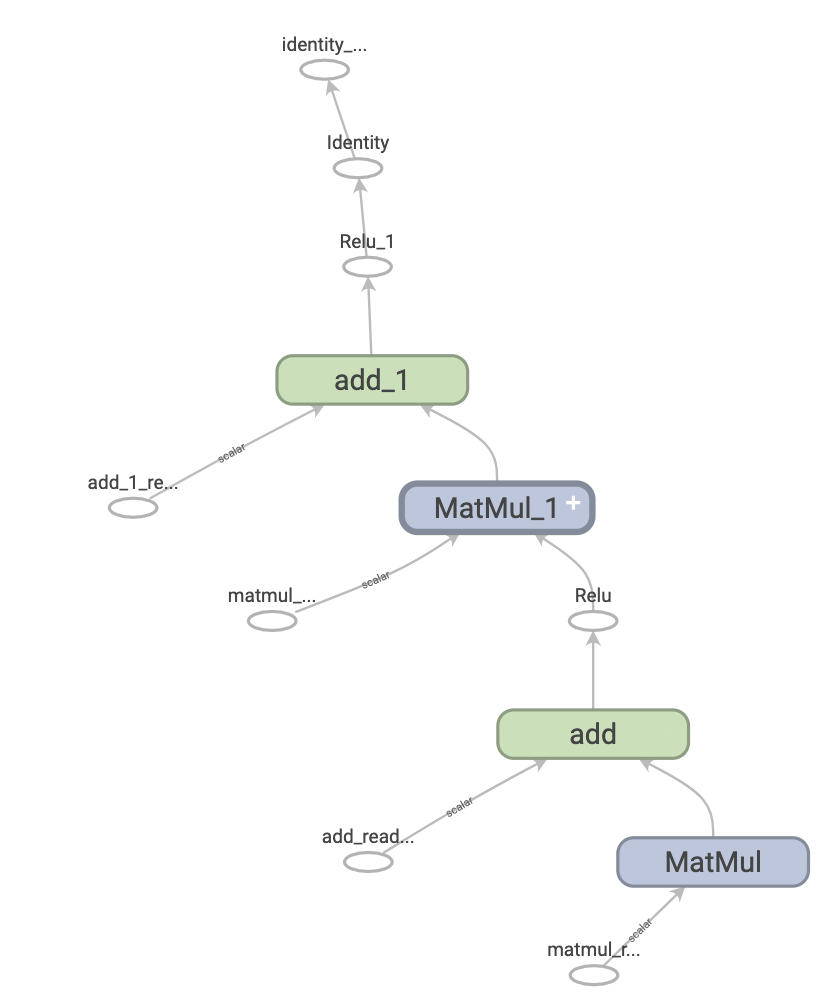
\includegraphics[width=\textwidth]{two-layer-network.png}
        \label{fig:sub2}
    \end{subfigure}
    \caption{Пример графа исполнения \textbf{Tensorflow}.}
    \label{fig:main}
\end{figure}

Становится очевидным, что разрыв между уровнями абстракции — от описания модели до низкоуровневой реализации — представляет собой незаполненную нишу, которую можно использовать для улучшения существующей инфраструктуры исполнения и оптимизации ML-программ.
Один из удачных примеров подобного подхода — проект LLVM, получивший широкое распространение и продолжающий активно развиваться.
Ключевым преимуществом LLVM является высокая модульность и гибкость его архитектуры.
Это достигается благодаря введению промежуточного представления (англ. Intermediate Representation, IR), которое используется как основа для множества этапов компиляции и оптимизации.

\textbf{LLVM IR} сохраняет семантику исходной программы, написанной на высокоуровневом языке, но одновременно обладает структурой, близкой к ассемблерному коду.
Такое сочетание делает IR мощным инструментом для анализа и преобразования программ на этапе, независимом от целевой архитектуры.
Одним из главных достоинств LLVM IR является возможность реализации архитектурно-независимых оптимизаций, применяемых до генерации финального машинного кода. К таким оптимизациям можно отнести:

\begin{itemize}
    \item распространение констант (constant propagation),
    \item разворачивание циклов (loop unrolling),
    \item  инлайнинг функций,
    \item переупорядочивание инструкций и устранение избыточных операций.
\end{itemize}

Важно отметить, что LLVM предоставляет расширяемую инфраструктуру, позволяя добавлять собственные типы, инструкции, метаинформацию и реализовывать пользовательские проходы оптимизации (passes).
Кроме того, LLVM IR активно используется в реализации оптимизаций, направляемых профилем выполнения (Profile-Guided Optimizations, PGO), где информация о поведении программы в реальных условиях позволяет проводить более эффективные преобразования.

Тем не менее, несмотря на выразительность и гибкость LLVM IR, он остается ориентированным на императивные языки общего назначения и ближе к низкоуровневой модели вычислений.
В условиях растущей сложности моделей машинного обучения, необходимости в высокоуровневых тензорных операциях, графовых представлениях и специфике разнообразных аппаратных ускорителей (GPU, NPU), возникает потребность в промежуточном представлении, способном отразить более абстрактные вычисления, сохраняя при этом поддержку всех преимуществ компиляторной инфраструктуры.

\subsection{Уровни абстракций и MLIR}

Именно по этой причине в апреле 2019 года был представлен новый проект от разработчиков LLVM, направленный на решение проблемы разрыва между уровнями абстракций в представлениях программ — MLIR.
\textbf{MLIR} (от англ. Multi-Level Intermediate Representation) представляет собой принципиально новый подход к описанию и трансформации высокоуровневых операций.
Само название — многоуровневое промежуточное представление — точно отражает основную идею проекта.
Используя модульную архитектуру LLVM, разработчики предложили расширяемую инфраструктуру, в рамках которой стало возможным создавать собственные уровни представления — так называемые диалекты (dialects).
Каждый диалект описывает специфический набор операций, типов и правил обработки, соответствующий определённому уровню абстракции.
Теперь, благодаря механизму lowering (понижение уровня представления), стало возможно последовательно преобразовывать программу с высокого уровня до низкоуровневого представления LLVM IR, контролируя и оптимизируя каждый этап компиляции.

Для современных фреймворков машинного обучения типичный процесс перехода по уровням абстракций выглядит следующим образом:
\begin{itemize}
    \item \textbf{TF} или \textbf{TFLite} - диалект уровня исходного кода моделей,
    \item \textbf{MHLO} или \textbf{TOSA} - диалект математических операций ML (присутствуют тензоры, батчи и др.),
    \item \textbf{LINALG} - диалект алгебры линейных операций (использует буферы вместо тензоров),
    \item \textbf{VECTOR} - диплект низкоуровневого векторного представления.
    \item \textbf{LLVM IR}
\end{itemize}


\begin{figure}[h]
\centering
\begin{overpic}[width=0.8\textwidth]{codegen-dialect-hierarchy.png}
\end{overpic}
\caption{Схема многоуровневого представления MLIR.}
\end{figure}

\textbf{Целью} данной работы является создание инструмента для \textbf{PGO} (Profile-Guided Optimization) в инфраструктуре MLIR, позволяющего проводить анализ участков исполнения программы, требующих непосредственной оптимизации.
Предлагается использовать существующие профилировщики программ машинного обучения и разработать расширение диалекта верхнего уровня за счёт добавления полей метаданных.
Такое отображение профиля исполнения на граф операций позволит принимать решения об оптимизации высокоуровневых операций на основе фактического поведения программы, при этом сохранив совместимость с широким набором существующих моделей.

\newpage
 %% Введение
    \section{Постановка задачи}
\label{sec:Chapter1} \index{Chapter1}

Необходимость вышеописанного инстремента в сущности очевидна, его наличие позволило бы детально инспектировать программы машинного обучения и быстро находить места, требующие оптимизаций.
В особенности с появлением новых вычислительных ускорителей и альтернативных архитектур очень актуальным становится вопрос об оптимизациях для исполнения на конкретных устройствах.
Это позволило бы значительно ускорить предкомпилированные модели, использующие оптимизации основанные на их же профиле исполнения.

Чтобы достичь этой цели, сформулируем задачу решаемую в рамках данной дипломной работы:

\begin{quote}
\textit{Разработка средства автоматического аннотирования промежуточного представления программ на основе профиля исполнения в рамках инфраструктуры MLIR}
\end{quote}

Поставлненная задача требует дополнительных пояснения, тк не может быть решена исходя из начальной формулировки.
Постараемся разбить задачу на более мелкие части и зададимся целью подробного описания их взаимосвязи.
Будем ранжировать также подзадачи в порядке убывающей важности, так чтобы сохранять акцент на поставленной задаче.
Рассмотрим каждую из сформулированных подзадач в отдельности:

\subsection{Расширение существующего диалекта/ов}

MLIR предоставляет широкие возможности как для создания собственных диалектов, так и для расширения уже существующих.
Однако, в отличие от классических объектно-ориентированных подходов, в MLIR отсутствует механизм прямого наследования диалектов, поскольку архитектура системы строится на принципах композиции.

Цель данной работы — получение расширенного промежуточного представления, способного не только сохранять профиль исполнения, но и обеспечивать доступ к этим данным на любом уровне абстракции после понижения (lowering).

Рассматривался подход создания обёрточного (proxy) диалекта, однако он оказался неприемлемым по ряду причин. Такой диалект создает дополнительный уровень представления, где каждый узел графа должен содержать информацию о соответствии операциям различных существующих диалектов.
Это потребовало бы ручного или автоматического "протягивания" метаданных через весь процесс lowering'а, что существенно усложняет архитектуру и увеличивает техническую сложность без значимых преимуществ.
По этой причине такой путь был отвергнут.

В данной работе основным и выбранным для реализации способом является создание интерфейса для основных операций.
Этот подход не привязан к конкретному диалекту, а лишь служит инструментом в рамках контекста выбранных для профилирования операций.
Небольшой участок кода поможет лучше понять структуру предлагаемого подхода:

\begin{lstlisting}[caption={Структура реализуемого интерфейса}]

class ProfiledOpInterface : public OpInterface<ProfiledOpInterface> {
    public:
    void attachProfileData(ProfileData data);
    ProfileData getProfileData();
    bool hasProfileData();
};

\end{lstlisting}

Важно подчеркнуть, что данный подход не накладывает жестких ограничений на целевой (инспектируемый) диалект и может быть реализован на произвольном уровне абстракции, соответствующем интересам анализа.
Кроме того, описанный паттерн органично интегрируется в модульную архитектуру MLIR, не нарушая ее принципов и не внося дополнительных межмодульных зависимостей.
Подробнее о конкретной реализации интерфейса и служебных структур в контексте аннотируемых метаданных можно ознакомться в секции~\nameref{sec:Chapter3}.

\subsection{Получение формата данных профилирования}

Следующей и не менее важной подзадачей является получение унифицированного формата данных после работы профилировщика.
В этой работе предлагается расширить возможности использования привычного для PGO оптимизаций в LLVM профилировщика perf.
На сегодняшний день интересующие нас фреймворки \textbf{Tensorflow}, \textbf{ONNX} и \textbf{PyTorch} предлагают готовые решения для сбора различной статистики выполнения высокоуровневых операций.

Типичный кусок кода написанный для сбора профиля исполнения модели:

\begin{lstlisting}[caption={Получение профиля с помощью утилиты фреймворка \textbf{Tensorflow}}]
    # Profiling options set
    options = tf.profiler.experimental.ProfilerOptions(
        ...
    )
    # Profiling start
    tf.profiler.experimental.start(log_dir, options=options)

    try:
        # Model run code
                ...
    finally:
        # Profiling stop
        tf.profiler.experimental.stop()
\end{lstlisting}

Согласно документации tensorflow-profile-plugin [см источник \cite{tf_profiler}] в настоящее время поддерживается следующий список устройств, в соответствующей конфигурации:

\begin{figure}[h]
\centering
\begin{overpic}[width=0.8\textwidth]{profiler-platforms.png}
\end{overpic}
\caption{Список поддерживаемых устройств и режимов работы профилировщика \textbf{TensorFlow}.}
\end{figure}

В рамках данной работы в качестве целевой платформы предлагается использовать \textbf{CPU}.
Важно отметить, что такой выбор не накладывает ограничений на область применимости разрабатываемого инструмента профилирования.

С появлением поддержки новых устройств в существующих профилировщиках, либо при использовании альтернативных решений, разработанных для отдельных устройств (например, Huawei NPU Ascend), потребуется изменить лишь этап предобработки входных данных, но не саму архитектуру обработки и анализа.
Такой уровень абстракции достигается за счёт использования промежуточного формата представления данных профиля в виде сериализованного файла \texttt{.json}.

Преимущества этого подхода, а также его реализация, будут подробно рассмотрены в секции~\nameref{sec:Chapter3}.

Последним замечанием к описанию подзадачи получения формата данных профиля будет представлен список возможностей \textbf{Tensorflow}.

\begin{itemize}
    \item Анализатор конвейера данных - анализирует эффективность загрузки и предобработки данных, помогает выявить узкие места в подаче данных в модель
    \item Статистика TensorFlow - собирает и отображает статистику выполнения операций, показывает время работы каждой операции и использование ресурсов
    \item Просмотрщик трассировки - визуализирует временную шкалу выполнения операций на процессоре и GPU, позволяет увидеть параллельность и простои
    \item Инструмент профилирования памяти - отслеживает использование памяти GPU и RAM, помогает оптимизировать потребление памяти и избежать переполнения
\end{itemize}

Каждый инструмент решает конкретные задачи оптимизации: от анализа загрузки данных до мониторинга распределенного обучения.
Второй и третий пункты из списка возможностей будут активно использованы в рамках выполнения практической части дипломной работы.

Подробнее о возможностях \texttt{TensorflowProfiler} и формате выходных данных будет рассказано в секции ~\nameref{sec:Chapter2}.

\subsection{Визуализация и анализ}

После получения формата профилированных данных и создания интерфейса взаимодействия с ними в рамках операций MLIR, формируется подзадача визуализации результатов профилирования на итоговом графе исполнения.
Данный этап является значимым, поскольку качество визуального представления профиля критически важно по следующим причинам:

\begin{itemize}
\item обоснование аналитических выводов;
\item обеспечение наглядности и интерпретируемости результатов;
\item возможность последующего применения визуализации при разработке оптимизаций.
\end{itemize}

Примером возможных преобразований могут являться трансформации графа, основанные на длительности выполнения операций.
Графическое представление последовательности вычислений в виде ориентированного графа с аннотациями, содержащими данные профиля, позволяет локализовать узлы с наибольшей нагрузкой.

В качестве иллюстрации представлен условный граф, демонстрирующий целевой формат визуализации:

\begin{figure}[h]
\centering
\begin{overpic}[width=\textwidth]{example.png}
\end{overpic}
\caption{Условный пример визуализации профиля исполнения.}
\end{figure}

Представленные в приложениях визуализации (см. секцию~\nameref{sec:Chapter5}) позволяют выполнить оценку полноты и корректности реализованного инструмента.
Кроме того, на основе профиля реальной модели выделяются участки, требующие приоритетного применения оптимизаций.

\newpage
 %% Постановка задачи
    \section{Обзор существующих решений}
\label{sec:Chapter2} \index{Chapter2}

\subsection{Введение в раздел}

В условиях стремительного развития технологий машинного обучения особую актуальность приобретает задача эффективного выполнения сложных моделей на разнообразных аппаратных платформах. Одним из ключевых компонентов современной инфраструктуры стал промежуточный язык представления MLIR (Multi-Level Intermediate Representation), который служит унифицирующим звеном между высокоуровневыми описаниями моделей и низкоуровневым оптимизированным кодом. Тем не менее, существующая реализация MLIR демонстрирует ограниченные возможности для интеграции данных о производительности, что существенно затрудняет процесс комплексного анализа и оптимизации промежуточного представления.
Целью данного обзора является систематический анализ современных подходов к профилированию машинного обучения, инструментам анализа и манипуляции MLIR, а также методам визуализации производительности. В рамках исследования рассматриваются профилировщики ML-моделей, инструменты анализа и модификации промежуточного представления, системы метаданных и подходы к визуализации результатов профилирования. Особое внимание уделяется выявлению возможностей автоматического аннотирования MLIR на основе данных профиля выполнения.
Методология анализа базируется на следующих критериях оценки:

\begin{itemize}
\item \textbf{Функциональность}: степень охвата задач профилирования и аннотирования промежуточного представления.
\item \textbf{Архитектурная совместимость}: уровень интеграции с инфраструктурой MLIR/LLVM.
\item \textbf{Масштабируемость}: способность эффективно работать с моделями большого размера.
\item \textbf{Расширяемость}: возможность кастомизации и добавления новых метрик.
\item \textbf{Применимость}: соответствие целевой платформе (CPU) и экосистеме TensorFlow.
\end{itemize}

Анализ проводится по категориям инструментов, после чего осуществляется сравнительный анализ, направленный на выявление ключевых пробелов и перспектив интеграции различных решений.

\subsection{Профилировщики машинного обучения}

\subsubsection{TensorFlow Profiler}
TensorFlow Profiler представляет собой комплексный инструмент для анализа производительности, интегрированный непосредственно в экосистему TensorFlow. Архитектура профилировщика основана на тесной интеграции с TensorFlow Runtime, что обеспечивает сбор метрик на уровне отдельных операций и ядер вычислений при поддержке различных вычислительных бэкендов, включая CPU, GPU и TPU. Выходные данные профилировщика формируются в формате trace events (JSON), содержащем структурированную информацию о времени выполнения, использовании памяти и утилизации вычислительных ресурсов. Такой формат позволяет проводить детальный анализ производительности на уровне отдельных операций модели.
Несмотря на широкие возможности, TensorFlow Profiler имеет ряд ограничений, существенных в контексте интеграции с MLIR: жесткая привязка к TensorFlow Runtime, отсутствие прямой поддержки промежуточного представления MLIR и сложность извлечения метрик для отдельных операций MLIR. Таким образом, применение данного инструмента ограничено рамками экосистемы TensorFlow.

\subsubsection{PyTorch Profiler}
PyTorch Profiler предлагает альтернативный подход к профилированию, основанный на использовании Autograd profiler для отслеживания прямого и обратного распространения, а также Kineto backend для низкоуровневого анализа производительности. Интеграция с TensorBoard обеспечивает интерактивную визуализацию результатов профилирования, включая поддержку распределённого профилирования для многоузловых конфигураций.
Однако применимость PyTorch Profiler к задачам, связанным с MLIR, ограничена различиями в архитектуре промежуточного представления и ориентацией на специфичные для PyTorch структуры данных.

\subsubsection{XLA Profiler и связь с MLIR}
Особый интерес представляет XLA (Accelerated Linear Algebra) Profiler, который демонстрирует тесную связь с MLIR в процессе генерации кода. XLA использует MLIR в качестве промежуточного представления, что создаёт основу для интеграции профильных данных. Промежуточное представление XLA HLO (High-Level Optimizer) может быть транслировано в MLIR, обеспечивая прослеживаемость от исходного графа TensorFlow до низкоуровневого кода.
XLA Profiler предоставляет возможности анализа на уровне операций HLO, исследования паттернов fusion и различных оптимизаций. Высокую актуальность данного инструмента для пайплайнов, основанных на MLIR, определяет общность инфраструктуры и возможность переноса подходов профилирования.

\subsubsection{Системные профилировщики}
Системные профилировщики, такие как Intel VTune Profiler, Linux perf и LLVM XRay, обеспечивают микроархитектурный анализ и низкоуровневое профилирование. Intel VTune Profiler позволяет выявлять узкие места (hotspot analysis), анализировать паттерны доступа к памяти и интегрироваться с ML-фреймворками через API. Linux perf использует sampling-based профилирование с генерацией flame graphs для визуализации, однако имеет ограничения при анализе высокоуровневых ML-операций.
LLVM XRay предоставляет функцию трассировки на уровне функций и демонстрирует потенциал для инструментирования кода, сгенерированного из MLIR, что особенно важно для связывания профильных данных с промежуточным представлением.

\subsection{Инструменты анализа и манипуляции MLIR}

\subsubsection{Базовые инструменты MLIR}
MLIR представляет собой гибридное промежуточное представление, поддерживающее множество требований в унифицированной инфраструктуре. Базовые инструменты MLIR включают \texttt{mlir-opt} для трансформации промежуточного представления с возможностью добавления пользовательских проходов (pass’ов), а также \texttt{mlir-translate} для конвертации между различными форматами, включая импорт TensorFlow SavedModel в MLIR.
\texttt{mlir-opt} обеспечивает расширяемую архитектуру для добавления новых оптимизационных проходов, что создаёт предпосылки для интеграции проходов, работающих с профильными данными. Тем не менее, существующие возможности \texttt{mlir-opt} ограничены в контексте интеграции динамических данных профилирования.

\subsubsection{Визуализация MLIR}
Инструмент \texttt{mlir-to-dot} предназначен для генерации представления MLIR-кода в формате GraphViz, обеспечивая статическую визуализацию структуры промежуточного представления. Основными ограничениями данного инструмента являются отсутствие поддержки метрик времени выполнения и цветового кодирования производительности, что существенно снижает его применимость для анализа производительности.
Альтернативные подходы включают разработку пользовательских проходов для генерации аннотированных графов и интеграцию с внешними инструментами визуализации, что требует значительных дополнительных усилий по разработке.

\subsubsection{Проекты на базе MLIR}
IREE (Intermediate Representation Execution Environment) представляет собой MLIR-based end-to-end компилятор и среду выполнения, который компилирует MLIR в исполняемый код со встроенными возможностями профилирования runtime. IREE обеспечивает инструментирование MLIR-проходов для анализа времени компиляции, что демонстрирует потенциал интеграции профилирования в инфраструктуру MLIR.
Основные ограничения IREE связаны с фокусом на задачах инференса, а не на детальном анализе производительности промежуточного представления. В сообществе MLIR обсуждается необходимость обеспечения прослеживаемости между компонентами сгенерированного кода и операциями входной спецификации.
XLA-MLIR обеспечивает интеграцию XLA-компилятора с MLIR, создавая предпосылки для переноса возможностей XLA-профилирования в контекст MLIR. ByteIR демонстрирует промышленное применение MLIR с опытом интеграции профилирования и оптимизаций.

\subsection{Метаданные и аннотации в MLIR}

\subsubsection{Системы метаданных MLIR}
MLIR предоставляет развитую систему метаданных, включающую типизированные атрибуты операций, информацию о местоположении (location) для отслеживания источника операций, а также traits и interfaces для определения свойств операций. Атрибуты представляют собой статические метаданные, которые могут быть расширены для включения профильных данных, однако их статическая природа ограничивает возможности работы с динамическими runtime-метриками.
Информация о местоположении в MLIR создаёт потенциал для связывания профильных данных с конкретными операциями промежуточного представления. Traits и interfaces обеспечивают возможности для определения профилируемых операций и расширения функциональности существующих диалектов.
\subsubsection{Опыт LLVM в Profile-Guided Optimization (PGO)}

LLVM предоставляет развитую инфраструктуру для оптимизации на основе профиля (PGO) с workflow \texttt{-fprofile-generate} / \texttt{-fprofile-use} и специализированным форматом профильных данных. Метаданные профиля включают branch weights, block frequencies и интеграцию с оптимизационными проходами.
Применимость LLVM PGO к MLIR ограничена различиями в уровне абстракции и необходимостью адаптации для ML-специфичных метрик, таких как время выполнения тензорных операций и характеристики использования памяти.

\subsubsection{Ограничения текущих подходов}

Анализ существующих подходов выявляет отсутствие стандартизированного формата профильных аннотаций в MLIR, ограниченную поддержку динамических метрик и необходимость ручной интеграции с профилировщиками, что создаёт значительные барьеры для практического применения.
Традиционные методы визуализации производительности включают flame graphs для иерархического представления времени выполнения и heatmaps для цветового кодирования метрик производительности. Flame graphs имеют ограничения при представлении графов операций ML из-за различий в структуре данных, тогда как heatmaps демонстрируют применимость к визуализации вычислительных графов.
TensorBoard Graph Visualization обеспечивает интерактивную визуализацию графов TensorFlow с интеграцией профильных данных через overlays, однако ограничена привязкой к формату TensorFlow. Netron служит универсальным визуализатором нейронных сетей, но не предоставляет интеграции с профильными данными.
Специфические требования к визуализации MLIR включают поддержку иерархической структуры (модули, функции, блоки), цветовое кодирование «горячих» операций, интерактивность для детального анализа метрик и масштабируемость для больших графов.

\subsubsection{Анализ пробелов}
Анализ выявляет критические пробелы в существующей инфраструктуре:
\begin{itemize}
\item Отсутствуют готовые решения для связки профилировщиков ML с промежуточным представлением MLIR.
\item Существующие инструменты не поддерживают цветовое кодирование производительности на уровне операций MLIR.
\item Метаданные MLIR не предназначены для работы с динамическими runtime-метриками.
\item Необходимость использования множества разрозненных инструментов для полного workflow.
\end{itemize}


\subsubsection{Научная и практическая значимость}
Разработка средства автоматического аннотирования MLIR на основе профиля выполнения обладает значимостью в следующих аспектах:
\begin{itemize}
\item Создание моста между профилированием ML-моделей и анализом промежуточного представления MLIR.
\item Предоставление данных для оптимизаций на основе профиля на уровне MLIR.
\item Визуализация производительности для быстрого выявления узких мест.
\end{itemize}

\subsubsection{Ожидаемые результаты}
Реализация предлагаемого средства обеспечит:
\begin{itemize}
\item Повышение эффективности анализа производительности ML-моделей.
\item Создание основы для будущих оптимизаций на основе профильных данных.
\item Расширение инструментария MLIR для практических задач анализа производительности.
\end{itemize}

\newpage %% Обзор существующих решений
    \section{Описание практической части}
\label{sec:Chapter4} \index{Chapter4}

Если в рамках работы писался какой-то код, здесь должно быть его
описание: выбранный язык и библиотеки и мотивы выбора, архитектура,
схема функционирования, теоретическая сложность алгоритма, характеристики
функционирования (скорость/память).

\newpage
 %% Описание практической части
    \section{Заключение}
\label{sec:Chapter4} \index{Chapter4}

В рамках данной работы было подробно рассмотрено современное решение для разработки компиляторов программ машинного обучения — MLIR.
Благодаря модульной и расширяемой архитектуре удалось интегрировать собственный пайплайн, который добавляет аннотации времени выполнения высокоуровневых операций.
Кроме того, в ходе работы были получены данные о выполнении операций на центральном процессоре с использованием TensorFlow Profiler, которые затем были сохранены в унифицированном формате (DAG).
Преимущество данного подхода было продемонстрировано на примере разработанной утилиты для визуального анализа последовательности произвольных событий, связанных с временем исполнения.
Все разработанные модули были объединены в единый инструмент, который предоставляет возможность автоматического аннотирования высокоуровневых операций собранной информацией о профилировании.
Сравнивая полученные результаты с перечнем поставленных целей, можно утверждать, что все цели работы были успешно достигнуты. Разработанное решение может быть использовано сторонними специалистами на практике для анализа и оптимизации программ машинного обучения с использованием PGO.

\newpage
 %% Заключение

    %% НЕ ТРОГАЙТЕ!!!
    \nocite{*}
    \bibliography{references}

    %% в зависимости от надобности подключаем раздел "Приложение"
    % \newpage
    % \section*{Приложение}
\addcontentsline{toc}{section}{Приложение}
\label{sec:Apendix} \index{Apendix}

Здесь необходимо написать приложение, которое вы должны придумать самостоятельно.

\end{document}
